% !TEX root = paper.tex
\section{PIOP Toolbox}
\subsection{Limb Reconstruction Check}
The \emph{Limb Reconstruction Check} takes 1 $n$-bit column $\col$ and $k$ columns $\col_0,\dots,\col_{k-1}$ each with $n/k$ bits and proves that each entry of $\col$ is the concatenation of the corresponding entries in $\col_0,\dots,\col_{k-1}$. We package this as the relation
\begin{displaymath}
\NPRelation_{\mathsf{Limb}} = \left\{\,
  \NPInstance = n,\;
  \NPInstancey = (\Oracle{\MLE{\col}}, \Oracle{\MLE{\col_0}}, \dots, \Oracle{\MLE{\col_{k-1}}}),\;
  \NPWitness = (\col, \col_0, \dots, \col_{k-1})
  \;\middle|\;
    \forall i,\, \col[i] = \sum_{j=0}^{k-1} 2^{(k-1-j)n/k} \col_j[i]
\,\right\}.
\end{displaymath}


\begin{DefinePIOP}{Limb Reconstruction Check}{limb-check}
    TODO
\end{DefinePIOP}

\subsection{Lookup Check}
The \emph{Lookup Check} takes two columns $\col_1$ and $\col_2$ and proves that every entry of $\col_1$ can be found in $\col_2$. We package this as the relation
\begin{displaymath}
\NPRelation_{\mathsf{Range}} = \left\{\,
  \NPInstance = n,\;
  \NPInstancey = (\Oracle{\MLE{\col_1}}),\;
  \NPWitness = (\col_1)
  \;\middle|\;
    \forall i,\, 0\leq \col[i] < 2^n
\,\right\}.
\end{displaymath}


\begin{DefinePIOP}{Lookup Check}{lookup-check}
    TODO
\end{DefinePIOP}


\subsection{Range Check}
The \emph{Range Check} takes a column $\col$ and proves that every entry of $\col$ is within an $n$-bit range. We package this as the relation
\begin{displaymath}
\NPRelation_{\mathsf{Range}} = \left\{\,
  \NPInstance = n,\;
  \NPInstancey = (\Oracle{\MLE{\col}}),\;
  \NPWitness = (\col)
  \;\middle|\;
    \forall i,\, 0\leq \col[i] < 2^n
\,\right\}.
\end{displaymath}


\begin{DefinePIOP}{Range Check}{range-check}
    TODO
\end{DefinePIOP}

\subsection{Bitwise AND}
The \emph{Bitwise AND check} takes three columns $\col_1, \col_2, \col_3$ containing $n$-bit values and proves that every entry of $\col_3$ is the bitwise AND of the corresponding entries in $\col_1$ and $\col_2$. We package this as the relation
\begin{displaymath}
\NPRelation_{\mathsf{BitwiseAND}} = \left\{\,
  \NPInstance = n,\;
  \NPInstancey = (\Oracle{\MLE{\col_1}}, \Oracle{\MLE{\col_2}}, \Oracle{\MLE{\col_3}}),\;
  \NPWitness = (\col_1, \col_2, \col_3)
  \;\middle|\;
    \forall i,\, \col_3[i] = \col_1[i] \land \col_2[i]
\,\right\}.
\end{displaymath}

\begin{figure}[h]
\centering
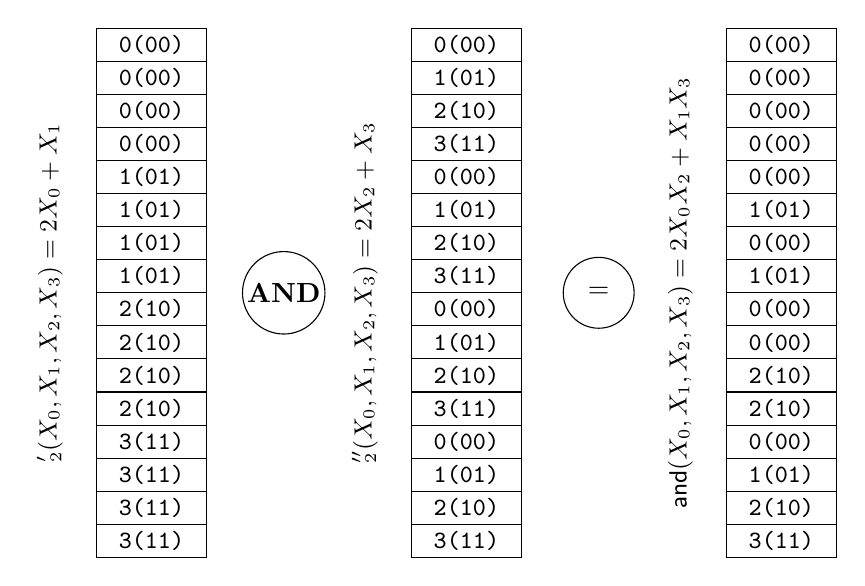
\begin{tikzpicture}[
  cell/.style={draw, minimum width=1.4cm, minimum height=0.42cm, font=\ttfamily\small, inner sep=1pt},
  op/.style={draw, circle, minimum size=0.9cm, font=\bfseries, inner sep=1pt, fill=white},
  collabel/.style={rotate=90, anchor=south, font=\small}
]
\def\cellH{0.42}
\def\colSep{4.0}
\foreach \v [count=\i from 0] in
  {0(00),0(00),0(00),0(00),1(01),1(01),1(01),1(01),2(10),2(10),2(10),2(10),3(11),3(11),3(11),3(11)}
  {\node[cell] (a\i) at (0, -\cellH*\i) {\v};}
\foreach \v [count=\i from 0] in
  {0(00),1(01),2(10),3(11),0(00),1(01),2(10),3(11),0(00),1(01),2(10),3(11),0(00),1(01),2(10),3(11)}
  {\node[cell] (b\i) at (\colSep, -\cellH*\i) {\v};}
\foreach \v [count=\i from 0] in
  {0(00),0(00),0(00),0(00),0(00),1(01),0(00),1(01),0(00),0(00),2(10),2(10),0(00),1(01),2(10),3(11)}
  {\node[cell] (c\i) at (2*\colSep, -\cellH*\i) {\v};}
\node[op] at (0.42*\colSep, -\cellH*7.5) {AND};
\node[op] at (1.42*\colSep, -\cellH*7.5) {$=$};
\node[collabel] at (-1.0, -\cellH*7.5) {$\idx'_2(X_0,X_1,X_2,X_3) = 2X_0 + X_1$};
\node[collabel] at (\colSep-1.0, -\cellH*7.5) {$\idx''_2(X_0,X_1,X_2,X_3) = 2X_2 + X_3$};
\node[collabel] at (2*\colSep-1.0, -\cellH*7.5) {$\MLE{\mathsf{and}}(X_0,X_1,X_2,X_3) = 2X_0X_2+X_1X_3$};
\end{tikzpicture}
\caption{The arithmetized truth-table for the bitwise AND function on n=2 bit inputs.}
\label{fig:bitwise-and-tt}
\end{figure}

To convince the verifier that each row of $\col_3$ is the bitwise AND of the corresponding rows of $\col_1$ and $\col_2$, the prover will convince the verifier that the concatenated rows of $\col_1, \col_2, \col_3$ can be looked up in a truth table encoding the bitwise AND function. More concretely,
\begin{DefinePIOP}{BitwiseAND}{bitwise-and}
    \begin{enumerate}[nosep]
        \item $\PIOPProver$ and $\PIOPVerifier$ invoke \cref{piop:range-check} on each of the three columns to check that they are all $n$-bit.
        \item $\PIOPVerifier$ samples three random field elements $r_1, r_2,r_3$ and sends them to $\PIOPProver$. 
        \item $\PIOPProver$ and $\PIOPVerifier$ invoke \cref{piop:lookup-check} to check that the concatenated column $\col' = r_1\col_1 + r_2\col_2 + r_3\col_3$ can be looked up in the column $\col'' = r_1\idx'_n+r_2\idx''_n+r_3\MLE{o}$ where 
        \begin{align*}
            \idx'_n(X_0,\ldots,X_{n-1}) &= \sum_{i=0}^{n-1} 2^{n-1-i} X_i, \\
            \idx''_n(X_0,\ldots,X_{n-1}) &= \sum_{i=0}^{n-1} 2^{n-1-i} X_{n+i}, \\
            \MLE{\mathsf{and}}(X_0,\ldots,X_{2n-1}) &= \sum_{i=0}^{n-1} 2^{n-1-i} X_iX_{n+i}.
        \end{align*}
    \end{enumerate}
\end{DefinePIOP}

